\section{Implementáció}
\subsection{A programról}
\paragraph{}A demó programmal egy jelenetet vizsgálhatunk, többféle átlátszósági technika lencséjén keresztül. A kamera egy szürke dobozban kering, melyben elszórtan különféle anyagi tulajdonságú gömbök, illetve különféle színű és intenzitású pontfények lebegnek.
\paragraph{}A technikákból a számbillentyűkkel(1-4) választhat a felhasználó. Kilépéshez az Escape billenytűt kell megnyomni.
\subsection{Részletek}
\subsubsection{Átlátszóság független részletek}
\paragraph{}A program felépítéseben a 3D Grafikus Rendszerek című tárgy laboranyagai jelentettek meghatározó inspirációt. Szerkezete objektum orientált. C++-ban íródott a GLFW, GLEW és GLM segédkönyvtárak felhasználásával. Implementálja még, bár jelenlegi állapotában nem használja az \textit{STB\_image} nevű fejlécfájlt textúrák képből történő betöltéséhez.
\paragraph{}Az árnyalást a max-Blinn módszerrel végzem, a vertex shader\index{vertex shader} ehhez állít elő adatokat, mint a fragmens\index{fragmens}\index{fragment} és a fények közötti eltolásvektor. A végső képet egy textúrából egy teljesképernyős négyszögre rajzolom.
\subsubsection{Alpha Blending}
\paragraph{}A \ac{GL} beépített keverését lineráis interpolációra állítottam.
\subsubsection{Depth Peeling}
\paragraph{}Ez a metódus a fent említett max-Blinn shader egy módosított változatát használja, mely a bejövő Z-buffer\index{Z-buffer}\index{depth buffer} adatok alapján elveti a fragmenseket. A kész képet négy menetből állítja elő, melyből az első a módosítatlan shaderrel készül. A keverést egy külön shader végzi.
\subsubsection{MBOIT}
\paragraph{}Jelenleg implementálatlan.
\subsubsection{WOIT}
\paragraph{}Jelenleg implementálatlan.

\newpage
\section{Tapasztalatok}
\subsection{Időbeosztás}
\paragraph{}Március végén-április elején álltam neki a demó program elkészítésének, bár ez később késeinek ígérkezett, ugyanis egyéb \-- egyetemi és más\-- kötelességeim miatt nem tudtam úgy haladni, mint szerettem volna. A tavaszi szünetet teljesen a lemaradás behozásával töltöttem.
\paragraph{}A következő héten segítséget kértem a konzulensemtől egy problémában, amit nem láttam át. Eme vizit közben beszéltük meg, hogy nem kell a félév végéig mindennel elkészülnöm, ha úgy is ebből a témából fogom készíteni a szakdolgozatomat.

\subsection{Kihívások}
\paragraph{}A többé-kevésbé titokzatos eredetű grafikai hibákkal meggyűlt s meggyűlik a bajom. Legfrissebb példa erre a \ref{img:tiger} képen látható probléma.

\begin{figure}[!b]
	\centering
	\label{img:tiger}
	\caption{Ismeretlen eredetű érdekes mintázat.}
	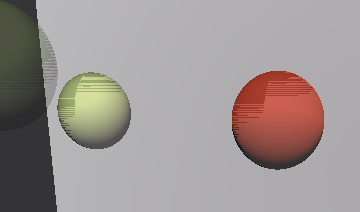
\includegraphics[width=300pt, keepaspectratio]{tigerprint.png}
\end{figure}
\section{Kitekintés}
\paragraph{}Természetesen a közeljövőben a MBOIT és WOIT implementációi következnek. A szakdolgozat keretében viszont felmerült már pár lehetőség:
\begin{itemize}
	\item Aizenshtein és társai felvetik egy egymenetes WOIT implementáció lehetőségét.
	\item Konzulensem ajánlotta, hogy a tárgyalt modern OIT egyikét bővítsem ki árnyékok megrajzolására.
\end{itemize}